% GENERAL INFORMATION: HardwareX is an open access journal established to promote free and open source designing, building and customizing of scientific infrastructure (hardware). For more details on best practices for sharing open hardware see http://www.oshwa.org/sharing-best-practices/

\documentclass[11pt, letterpaper]{article}
\usepackage[utf8]{inputenc}
\usepackage[margin=1in]{geometry}
\usepackage{titlesec}
\usepackage{tabu}
\usepackage{enumitem}
\usepackage{amssymb}
\usepackage{graphicx}
\usepackage{hyperref}
\usepackage[square,numbers,sort&compress]{natbib}
\newlist{selectlist}{itemize}{2}
\setlist[selectlist]{label=$\square$,leftmargin=*,noitemsep,topsep=0pt}

% Set up the section label formatting
\titleformat{\section}[block]{\hspace{1em}\bfseries}{\thesection.}{0.5em}{} 
\titleformat{\subsection}[block]{\hspace{1em}}{\thesubsection}{0.5em}{}

\begin{document}
% Create the title block
\begin{flushleft}

% Remove all text in italics when filling out the template and replace with your manuscripts corresponding text in regular font.
% \textit{Text in italics are template instructions. Remove and replace all instructions with regular font text.}

\setlength{\parindent}{0pt}
\setlength{\parskip}{10pt}
% \textbf{\large HardwareX article template}

%Insert title
%Max. 20 words. A good title should contain the fewest possible words that adequately describe the content of a paper.
\textbf{Title:} A portable wave tank and wave energy converter for dissemination and outreach

%Insert Authors
\textbf{Authors:} \textit{Author one, author two, and author three}

%Insert Affiliations
\textbf{Affiliations:} Sandia National Laboratories, University of New Mexico

%Insert Contact Email
%Include institutional email address of the corresponding author
\textbf{Contact email:} rcoe@sandia.gov

%Insert Abstract
%Max. 200 words. Remember that the abstract is what readers see first in electronic abstracting and indexing services. This is the advertisement of your article. Make it interesting, and easy to be understood. Be accurate and specific, keep it as brief as possible.
\textbf{Abstract:} Wave energy converters are a nascent energy generation technology that harness the power in ocean waves.
To assist in communicating both fundamental and complex concepts of wave energy, a small scale portable wave tank and wave energy converter have been developed.
The system has been designed using commercial off-the-shelf components and the all design hardware and software are openly available for replication.

%Insert Keywords
% At least 3 keywords. There is no limit on the no. of keywords you can list. Please remember that effective keywords should not repeat words appearing in your title, and should be neither too general nor too narrow.
\textbf{Keywords:} wave energy, educational, outreach

\textbf{Specifications table:}

\tabulinesep=1ex
\begin{tabu} to \linewidth {|X|X[3,l]|}
\hline  \textbf{Hardware name} & Sandia Interactive Wave Energy Education Display (SIWEED)
  %Please specify the name of the hardware that you invented / customized
  \\
  \hline \textbf{Subject area} & %
  % Please state the subject area most relevant to the original community for which this hardware was developed. Example subject areas are listed below.
  \begin{itemize}
  % \item \textit{Engineering and Material Science}
  % \item \textit{Chemistry and Biochemistry}
  % \item \textit{Medical (e.g. Pharmaceutical Science)}
  % \item \textit{Neuroscience}
  % \item \textit{Biological Sciences (e.g. Microbiology and Biochemistry)}
  % \item \textit{Environmental, Planetary and Agricultural Sciences}
  \item \textit{Educational Tools and Open Source Alternatives to Existing Infrastructure}
  % \item \textit{General}
  \end{itemize}
  \\
  \hline \textbf{Hardware type} &
  \begin{itemize}
  % \item \textit{Imaging tools}
  % \item \textit{Measuring physical properties and in-lab sensors}
  % \item \textit{Biological sample handling and preparation}
  % \item \textit{Field measurements and sensors}
  \item \textit{Electrical engineering and computer science}
  \item \textit{Mechanical engineering and materials science}
  \item \textit{Other (please specify) - Ocean engineering}
  \end{itemize}
  \\ 
\hline \textbf{Open source license} &
  %Please specify the open source license. For more details see the guide to authors.
  GNU GENERAL PUBLIC LICENSE
  \\
\hline \textbf{Cost of hardware} &
  \textit{\$7736 - Approximate cost of hardware (complete breakdown included in the Bill of Materials).}
  \\
\hline \textbf{Source file repository} & 
  % Link to the source file repository, e.g. https://osf.io/q3nr5/ 
  https://github.com/SNL-WaterPower/siweed
\\\hline
\end{tabu}
 
\end{flushleft}
% create the main body of the paper

\section{Hardware in context} % Include a short description of the hardware, putting into context of similar open hardware and proprietary equipment in the field.
The SIWEED is a small scale wave tank that is designed to be portable and serve in outreach and dissemination of wave energy research.
The development of this system was inspired by previous research at Sandia National Labs in the areas of wave energy converter (WEC) device and control design and testing.
Specifically, the SIWEED demonstrates the causal feedback control and device design principles described in \citet{Bacelli2020} and \citet{Coe2020a}.


A wide variety of similar educational wave tanks and tow tanks have been built, but few have been documented.
\citet{unger2006creating} reworked a tow tank at MIT to enable remote operation via the internet.
\citet{Trust2015} created a tank with a similar size and objective, but oriented at demostrating the effectiveness of coastal flood controls.
There seem to be two major iterations, one electrically driven by a paddle like wave maker, and one plunger type driven mechanically by hand. 
That team has also make multiple similar hydraulic flume tanks for demonstration purposes.
\citet{Ivan2016} has an educational wave tank on display in the National Museum of Scotland, but the waves do not explicitly interact with any bodies on the surface. 
%\citet{Y.H.Yu} Made a wave tank to study floating- point absorbers as wave energy converters, showing similarities to this project, but they use a flap-type wavemaker, and their tank is much larger and not portable.

This is a novel expansion on similar small-scale educational wave tanks, as the user is able to control both the waves and the WEC device, and the wave maker is driven by a ballscrew.
The parameters of the wave are also much more controllable in this project than in similar small wave tanks.
The primary intended audience is college students and above, but there is implemented functionality to run a simplified version of the GUI for lower age groups.


\section{Hardware description} % Describe the hardware, highlighting the customization rather than the steps of the procedure. Highlight how it differs/which advantage it offers over pre-existing methods. For example, how could this hardware: be compared to other hardware in terms of cost or ease of use, be used in the development of further designs in a particular area, and so on. Add 3-5 bulleted points to broadly explain to other researchers how the hardware could be potentially useful to them, for either standard or novel laboratory tasks, inside or outside of the original user community.
The SIWEED is composed of a 1.5\,m $\times{}$ 0.3\,m $\times{}$ 0.5\,m acrylic tank, filled to roughly 0.3\,m deep, housing a vertical plunger style wave maker (see, e.g., \cite{hyun1976simplified}), and a single body WEC modeled on the WaveBot~\cite{Coe2016a}.
A system diagram is shown in \figurename~\ref{fig:siweed_layout}.
\begin{figure}[tb]
  \centering
  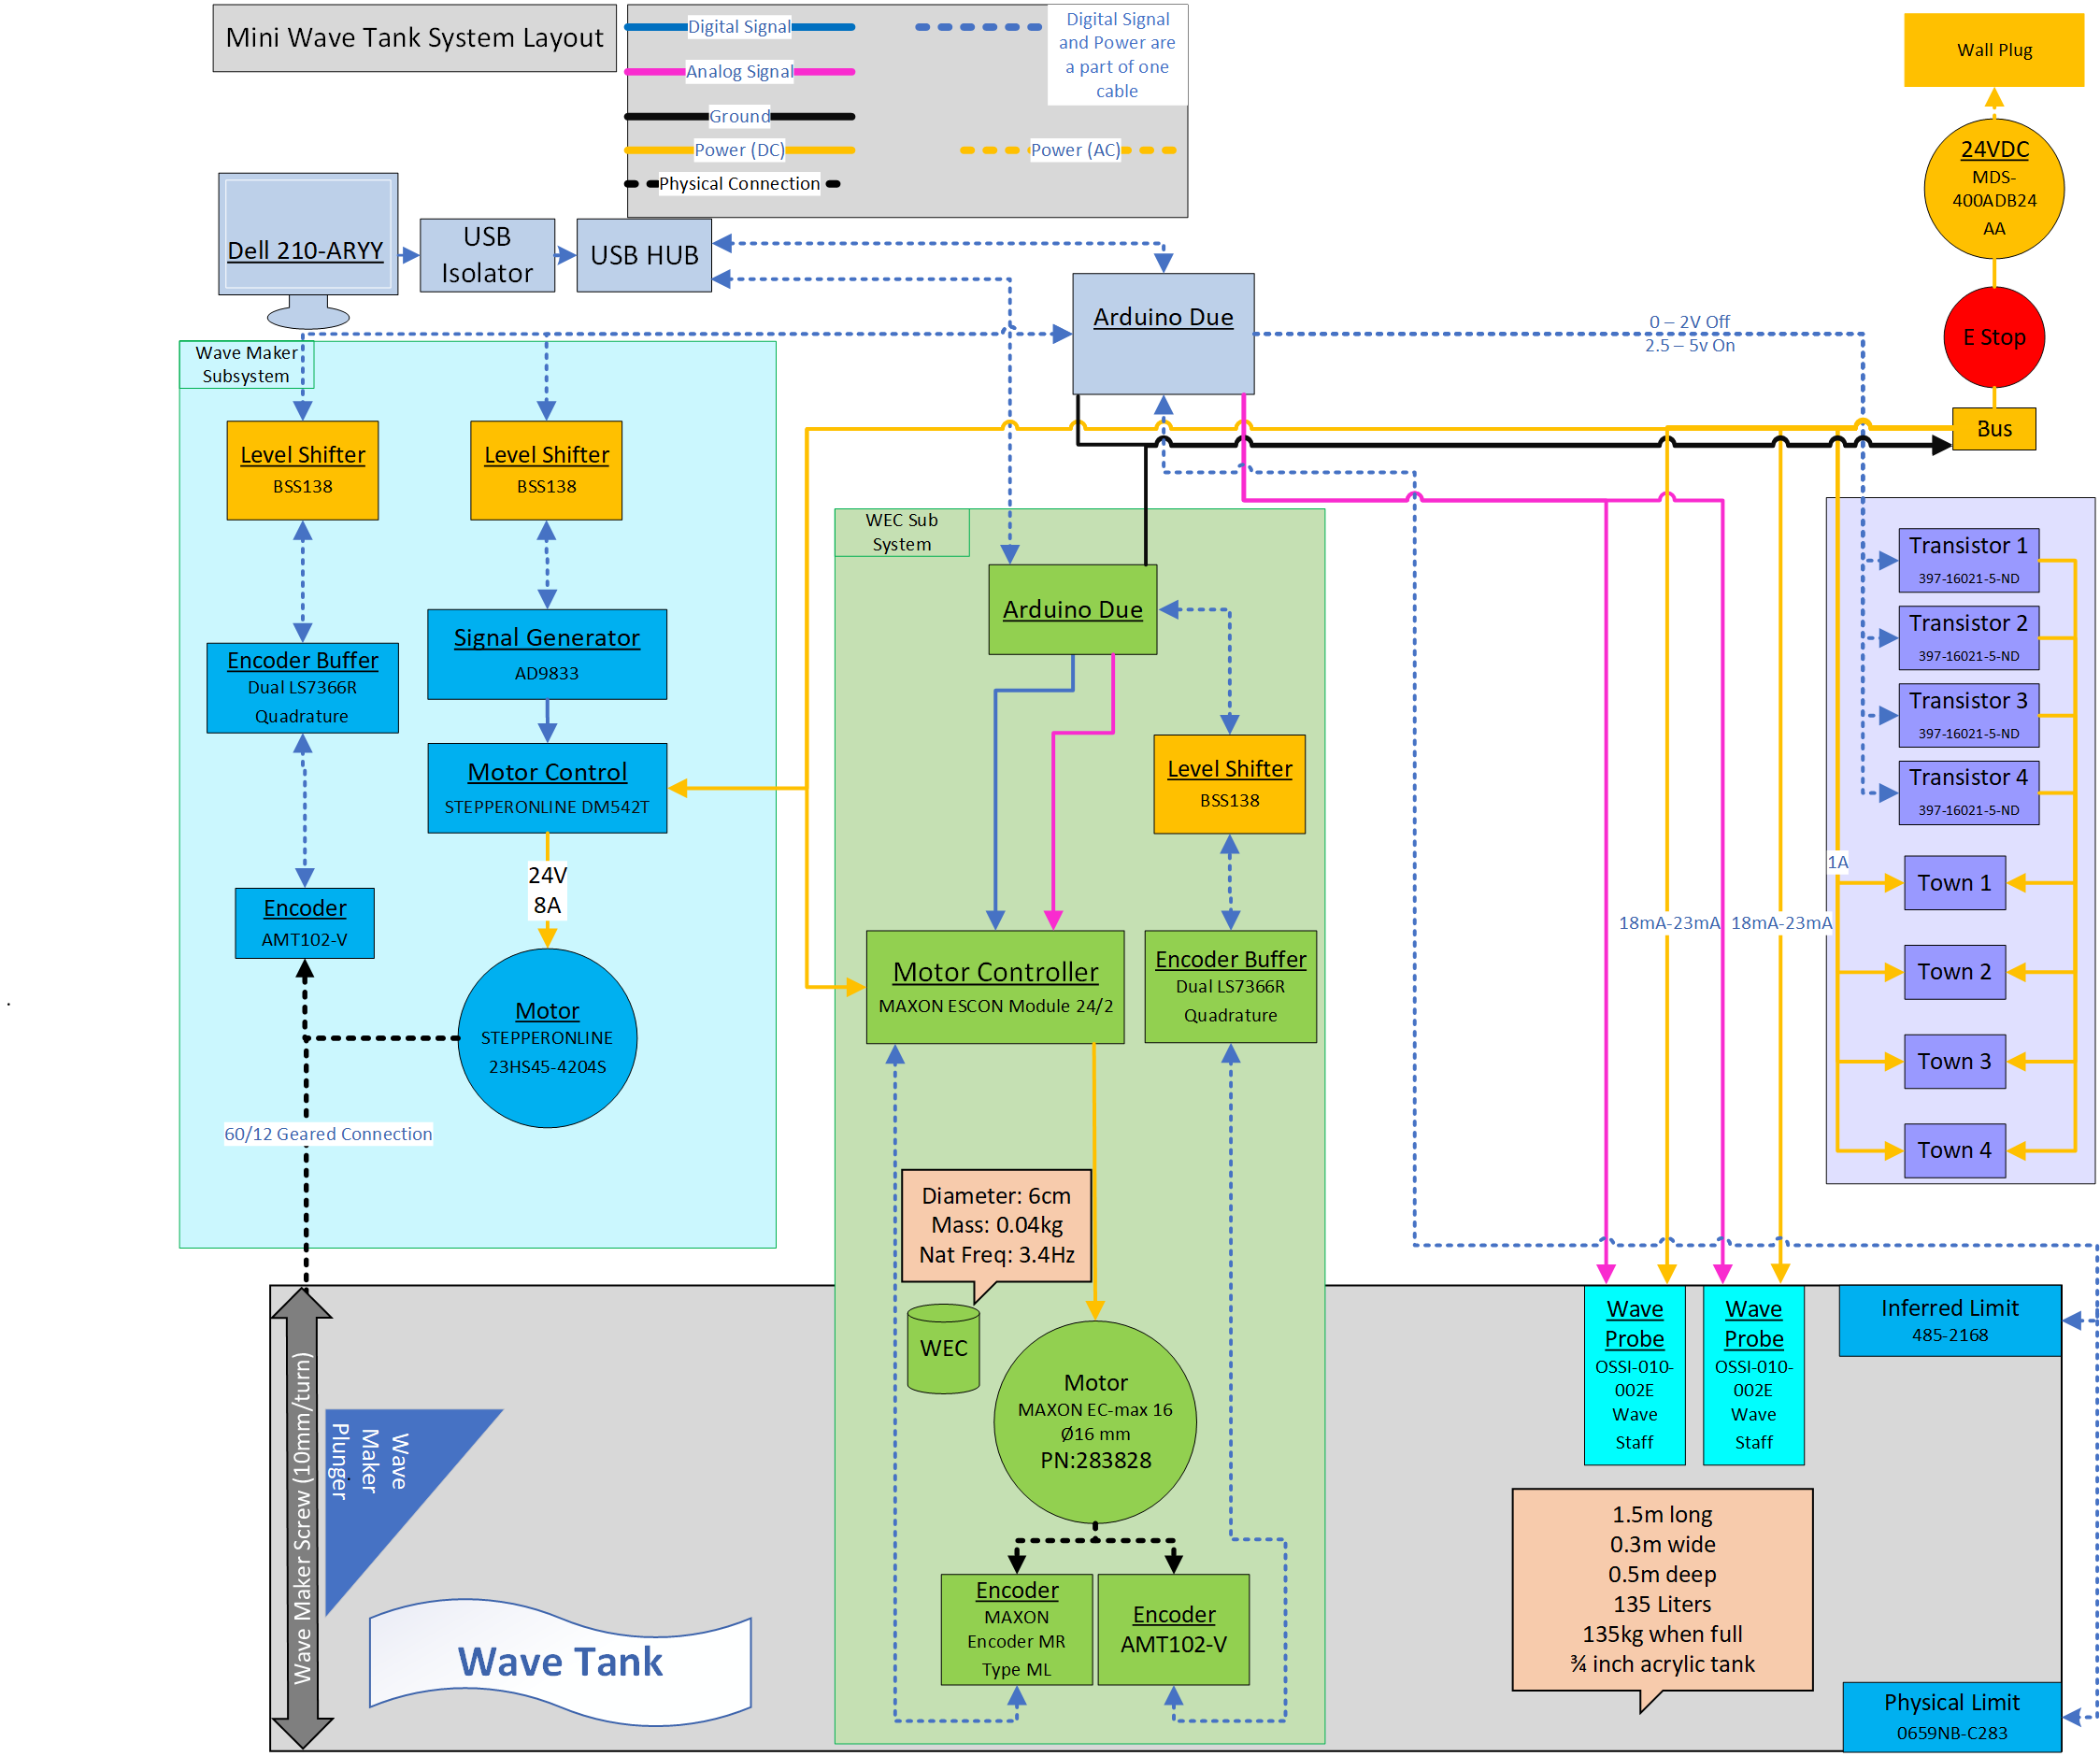
\includegraphics[width=1\textwidth]{diagrams/System Layout.png}
  \caption{System Layout Diagram.}
  \label{fig:siweed_layout}
\end{figure}
The system is controlled by a Windows PC running a graphical user interface (GUI) developed using Processing\footnote{\url{https://processing.org}} and the controlP5 library\footnote{\url{http://www.sojamo.de/libraries/controlP5/}}.
A screen shot of the GUI is shown in \figurename~\ref{fig:siweed_guiScreenShot}.
It is divided into three sections: The left instructional side, ``Mission Control", and ``System Status".

\begin{figure}[tb]
  \centering
  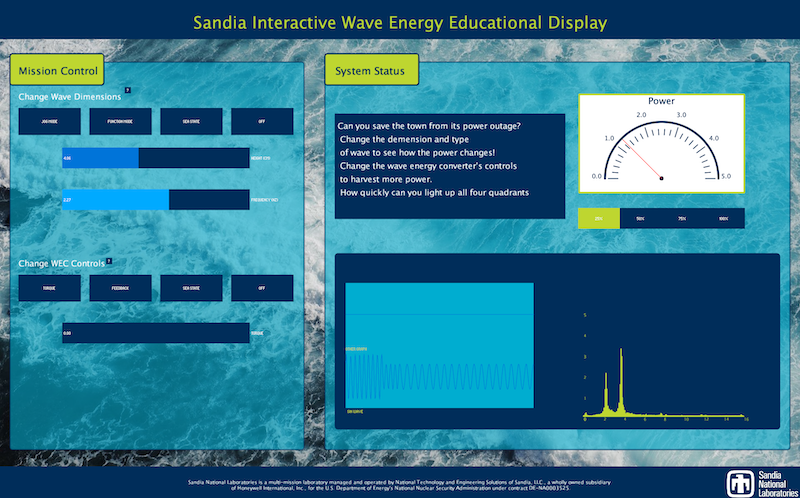
\includegraphics[width=1\textwidth]{diagrams/siweed_guiScreenShot.png}
  \caption{Graphical user interface (GUI) screenshot.}
  \label{fig:siweed_guiScreenShot}
\end{figure}

The left side of the ``Mission Control" section of the GUI pertains to control of the wave maker, which allows the user to switch between operational modes (``jog,'' ``function,'' ``sea state,'' and ``off'') and set the relevant parameters.
If, for example, the system is in ``sea state'' mode, the user can set the significant wave height ($H_s$), peak frequency ($f_p$), and peakedness factor ($\gamma$) for a JONSWAP wave spectrum.

The right side of the ``Mission Control" section of the GUI  contains controls for the WEC, which can be set into ``torque'' mode; in which the user directly sets a commanded torque, ``feedback'' mode; where proportional and integral feedback factors can be set by the user; ``multi-sine'' mode, which allows for open-loop multi-sine signals to be set by the user; and ``off.''

The ``System Status" section shows two plots, one for the WEC and one for the wave maker, with each allowing the user to choose what data is plotted. 
Below the plots are an FFT of the generated waves, and a radial meter that displays the hypothetical generated power of the WEC.

Two Arduino Due microcontrollers are used to control and acquire signals from the WEC and wave maker.

A number of key factors of SIWEED are:

\begin{itemize}
  \item \textbf{Open-source and documented design:} To our knowledge, the SIWEED is the first educational wave tank and WEC system to be fully documented with an open-source design and software package.
  This will enabled interested researchers and students to efficiently develop replicates and variations of the SIWEED design for their own purposes.
  \item \textbf{Portability:} To allow for transport to conferences and outreach events, the SIWEED has been specifically designed to allow for easy transportation.
  \item \textbf{WEC control:} In addition to demonstrating the physics of ocean waves, the SIWEED allows users to interact with a WEC control system to better understand the principles of reactive feedback control to maximize power absorption for the waves.
  \item \textbf{Student-led design:} The SIWEED project has been a student-led design project involving XX undergraduate engineering students.
  \item \textbf{Curriculum:} The SIWEED repository includes a curriculum for students K-12 based on the Next Generation Science Standards \cite{NextGenScience2021}. 
The repository contains a presentation and a document intended to be given to the teacher beforehand. 
The presentation explains water power and Sandia National Labs' role within it, and then goes into more detail about wave energy converters and how the SIWEED demonstration works.
The teacher resources document contains general information about the project, and a multitude of resources surrounding wave energy education, including videos, worksheets, vocabulary words, general topics, and Next Generation Science standards for each grade level.
\end{itemize}

\section{Design files}
%The complete design files must be either uploaded to an approved online repository, uploaded at the time of submission on the online Elsevier submission interface as supplementary materials (CAD files, videos…), or included in the body of the manuscript (e.g. figures). The two approved online repositories are Mendeley Data and the Open Science Framework (OSF instructions).
% Mendeley data: https://data.mendeley.com/
% Open Science Framework: https://osf.io/
% Open Science Framework HardwareX instructions: https://osf.io/wgk7q/wiki/home/
% > CAD files. Authors are encouraged to use free and open source software packages for creating the files. For CAD files, OpenSCAD, FreeCAD, or Blender are encouraged, but if not available source files from proprietary CAD packages such as Autocad or Solidworks and other drawing packages are acceptable.
%OpenSCAD: http://www.openscad.org/
% > 3D printing. Supplementary files that facilitate the digital replication of the devices are encouraged. For example, STL files for 3-D printing components. We recommend uploading CAD files to the NIH 3D Print Exchange as Custom Labware and providing a link to the location.
%NIH 3D Print Exchange: http://3dprint.nih.gov/
% > Electronics. PCB layouts and other electronics design files can be uploaded to the Open Hardware Repository or other repositories .
%Open Hardware Repository: http://www.ohwr.org/
% > Software and firmware. All software files used in the design and operation of the hardware should be included in the repository. Provide a description of software and firmware and use extensive comments in the code.

%\textit{The complete design files must be either uploaded to an approved online repository, uploaded at the time of submission on the online Elsevier submission interface as supplementary materials [CAD files, videos,\dots], or included in the body of the manuscript [e.g. figures]. The two approved online repositories are Mendeley Data and the Open Science Framework [OSF instructions]. Mendeley data: https://data.mendeley.com/ Open Science Framework: https://osf.io/ Open Science Framework HardwareX instructions: https://osf.io/wgk7q/wiki/home/
%\begin{itemize}
%\item CAD files. Authors are encouraged to use free and open source software packages for creating the files. For CAD files, OpenSCAD, FreeCAD, or Blender are encouraged, but if not available source files from proprietary CAD packages such as Autocad or Solidworks and other drawing packages are acceptable. OpenSCAD: %http://www.openscad.org/
%\item 3D printing. Supplementary files that facilitate the digital replication of the devices are encouraged. For example, STL files for 3-D printing components. We recommend uploading CAD files to the NIH 3D Print Exchange as Custom Labware and providing a link to the location. NIH 3D Print Exchange: http://3dprint.nih.gov/
%\item Electronics. PCB layouts and other electronics design files can be uploaded to the Open Hardware Repository or other repositories. Open Hardware Repository: http://www.ohwr.org/
%\item Software and firmware. All software files used in the design and operation of the hardware should be included in the repository. Provide a description of software and firmware and use extensive comments in the code.
%\end{itemize}
%}
\subsection{Design Files Summary}
% Please include a summary of all design files for your hardware by filling rows of the table below

\tabulinesep=1ex
\begin{tabu} to \linewidth {|X|X|X[1.5,1]|X[1.5,1]|}
\hline
\textbf{Design filename} & \textbf{File type} & \textbf{Open source license} & \textbf{Location of the file} \\\hline
%Insert design files
\textit{Design file 1} & \textit{e.g. CAD file, figures, videos} & \textit{All designs must be submitted under an open hardware license. Enter the corresponding open source license for the file.} & \textit{Enter a link to the online location or the sentence: ``available with the article'', as appropriate}  \\\hline
\textit{CAD} & XX& \dots & location \\\hline
\textit{Functional CAD} & XX & \dots & \dots \\\hline
\textit{Plunger CAD?} & XX & \dots & \dots \\\hline
\textit{miniWEC dimensions?} & XX & \dots & \dots \\\hline
\textit{Processing sketches} & XX & \dots & \dots \\\hline
\textit{Arduino sketches} & XX & \dots & \dots \\\hline
% Design file 3 & File type & License & Link \\\hline

\end{tabu}

% For each design file listed in the summary above, include a short description of the file below (one or two sentences)
\textit{For each design file listed above, include a short description of the file here (one or two sentences)}

\section{Bill of materials}
% For a complex Bill of Materials, the complete Bill of Materials (editable spreadsheet file e.g., ODS file type or PDF file) can be uploaded in an open access online location such as the Open Science Framework repository. Include the link here. Alternatively, the Bill of Materials can be uploaded at the time of submission on the online Elsevier submission interface as supplementary material.

% > To make it easy to tell which item in the Bill of Materials corresponds to which component in your design file(s), use matching designators in both places, or otherwise explain the correspondence.

% > For material type, select from: Metal, semi-conductor, ceramic, polymer, biomaterial, organic, inorganic, composite, nanomaterial, semiconductor, non-specific, or other  
The complete Bill of Materials can be found here: XX-put link here before uploading. Note that a SIWEED system can be assembled with any tank on hand (e.g., a fish tank) and any Windows PC capable of running the Processing IDE; as these components can contribute significantly to system cost, the BOM lists the tank and computer separately from the remainder of the components.
%\textit{For a complex Bill of Materials, the complete Bill of Materials (editable spreadsheet file e.g., ODS file type or PDF file) can be uploaded in an open access online location such as the Open Science Framework repository. Include the link here. Alternatively, the Bill of Materials can be uploaded at the time of submission on the online Elsevier submission interface as supplementary material.}
%\begin{itemize}
%\item \textit{To make it easy to tell which item in the Bill of Materials corresponds to which component in your design file(s), use matching designators in both places, or otherwise explain the correspondence.}
%\item \textit{For material type, select from: Metal, semi-conductor, ceramic, polymer, biomaterial, organic, inorganic, composite, nanomaterial, semiconductor, non-specific, or other} 
%\end{itemize}
%
%\tabulinesep=1ex
%\begin{tabu} to \linewidth {|X|X|X|X|X|X|X|}
%\hline
%\textbf{Designator} & \textbf{Component} & \textbf{Number} & \textbf{Cost per unit currency} & \textbf{Total cost} & \textbf{Source of materials} & \textbf{Material type} \\\hline
%%Insert items here
%\textit{Designator} & \textit{Name of Component 1} & \textit{Number of units} & \textit{Cost per unit} & \textit{Total cost} & \textit{Source} & \textit{Material type} \\\hline
%\end{tabu}

\section{Build instructions}
%Provide detailed, step by step instructions for the construction of the reported hardware include all necessary information for reproducing the submitted hardware.
% > Explain and, when possible, characterize design decisions. Including design alternatives if they exist. 
% > Use visual instructions such as schematics, images, and videos. 
% > Clearly reference design files and component parts described in the Design File Summary and Bill of Materials. 
% >Highlight potential safety concerns that may arise

Using the System Layout diagram in \figurename~\ref{fig:siweed_layout}, the bill of materials, and other dimensions listed in this document, a functionally similar version of this wavetank can be reconstructed. Many parts can be substituted with similar ones, such as the laptop, transistors, power supply, or the tank itself. Software specific hardware, such as the Arduinos or Encoder Buffers should not be substituted. 
Software setup:
\begin{itemize}
\item Download the latest version of Arduino IDE and Processing IDE.
\item Download the Master SIWEED Repository.
\item Change the Sketchbook Location for the Arduino IDE to \textbackslash siweed\textbackslash Arduino.
\item Change Sketchbook Location for the Processing IDE to \textbackslash siweed\textbackslash Processing.
\item Change Arduino IDE board to ``Arduino Due Programming Port".
\item Upload the sketches to the Arduinos.
\item A more detailed version of these instructions can be found in the README file of the repository.
\end{itemize}

\section{Operation instructions}
%Provide detailed instructions for the safe and proper operation of the hardware. 
%> Step-by-step operational instructions for operating the hardware. 
%> Use visual instructions as necessary. 
%> Highlight potential safety hazards.

After performing the setup described in the build instructions, the project can be operated as follows:
\begin{itemize}
\item Power on the wavetank, ensuring any kill switches are closed, and any pinch points are clear.
\item Open processing.exe.
\item File $>$ Open $>$ siweedGUI.pde 

(Ex: C\textbackslash Users\textbackslash user\textbackslash Documents\textbackslash GitHub\textbackslash siweed\textbackslash Processing\textbackslash siWeedGUI\textbackslash siweedGUI.pde) 
\item (optional)Edit modifiers. These are booleans at the top of the code that will do things like enable basic mode, debugging, or data logging.
\item Click ``Run".
\item The GUI will open, allow some time for it to load.
\item In the console, which will either be in the GUI, made visible by pressing the console button in the bottom right corner, or in the Processing console, depending on your boolean modifiers, unit tests should be visible that can be used to verify that everything is functioning properly.
\end{itemize}

\section{Validation and characterization}
%Demonstrate the operation of the hardware and characterize its performance over relevant critical metrics
%> Demonstrate the use of the hardware for a relevant use case. 
%> If possible, characterize performance of the hardware over operational parameters. 
%> Create a bulleted list that describes the capabilities (and limitations) of the hardware. For example consider descriptions of load, operation time, spin speed, coefficient of variation, accuracy, precision and etc. 

\begin{itemize}
\item \textbf{Torque constant verification:} 
The factory torque constant was verfied by logging the position and current of the free floating WEC while commanding a slow sinusoidal current.
The position displacement time series was converted to a time series of the applied physical torque with the following equation:
%\linebreak
\[\tau=\sigma*\gamma *d* \pi*r^2\]
%\linebreak
Where $\tau$ is torque, $\sigma$ is the radius of the pinion gear, $\gamma$ is the specific weight of water, d is the displacement of the buoy in the water, and r is the radius of the buoy.
%Torque = pinon radius (M)*  [9810(N/m^3)*pos(m)*pi*radius(m)^2]
It is important to note that the torque values at this point did not account for friction or hysteresis.
Plotting this torque data against the recorded commanded current values gives  \figurename~\ref{fig:TorqueConstant}.
The fit1 line represents the best linear fit of the entire data set, but the data points at the highest and lowest currents are affected more significatntly by static friction, so omitting them from the data set improves the torque constant estimation, as shown with the fit2 line in \figurename~\ref{fig:TorqueConstant}.
\begin{figure}[tb]
  \centering
  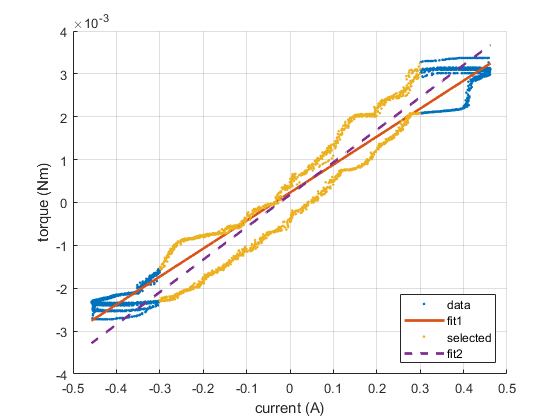
\includegraphics[width=0.5\textwidth]{diagrams/TorqueConstant.jpeg}
  \caption{Torque vs commanded current, with linear fits of the entire and partial data set.}
  \label{fig:TorqueConstant}
\end{figure}
This provides an estimated torque constant of about 7.52mNm/A, which is within 4\% of the factory stated constant of 7.8mNm/A.
\linebreak
Since torque is being estimated from displacement and the frequency is low (inertial and viscous effects are small), the friction shows up as a "constant" offset from the ideal torque constant and doesn't affect the slope.
This allows the friction to be seen as half the offset between the data points as the wave maker moves up, and the points as it moves down. 
Plotting the torque error using the calculated torque constant against the current gives \figurename~\ref{fig:TorqueError}.
\begin{figure}[tb]
  \centering
  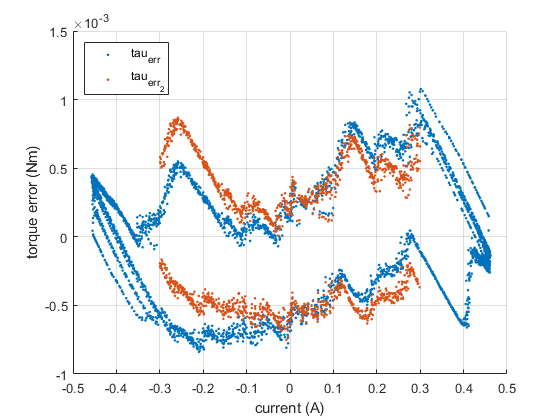
\includegraphics[width=0.5\textwidth]{diagrams/TorqueError.jpeg}
  \caption{Torque error vs commanded current.}
  \label{fig:TorqueError}
\end{figure}
The average offset shows that the friction is about 0.45mNm.

\item \textbf{Wave Probes:}
The readings from the wave probes could be verified by attaching them to the wave maker, which has a very precise encoder that allows for accurate changes in displacement. 
Moving the wave maker with the wave probe attached and comparing the displacement data from both of them was used to make sure the wave probe was providing accurate readings. 
\item \textbf{WEC feedback control} - XX
\end{itemize}

\section{Declaration of interest}
Declarations of interest: none
% a statement must be included even if there is no conflict of interest
% All authors must disclose any financial and personal relationships with other people or organizations that could inappropriately influence (bias) their work. Examples of potential conflicts of interest include employment, consultancies, stock ownership, honoraria, paid expert testimony, patent applications/registrations, and grants or other funding. Authors must disclose any interests in a summary declaration of interest statement in the manuscript file. If there are no interests to declare then please state this: 'Declarations of interest: none'. This summary statement will be ultimately published if the article is accepted. More information.}

\section*{Acknowledgment}
Sandia National Laboratories is a multi-mission laboratory managed and operated by National Technology and Engineering Solutions of Sandia, LLC., a wholly owned subsidiary of Honeywell International, Inc., for the U.S. Department of Energy's National Nuclear Security Administration under contract DE-NA0003525. This paper describes objective technical results and analysis. Any subjective views or opinions that might be expressed in the paper do not necessarily represent the views of the U.S. Department of Energy or the United States Government.

% \section{Human and animal rights}

% \textit{
% \begin{itemize}
% \item If the work involves the use of human subjects, the author should ensure that the work described has been carried out in accordance with the appropriate ethical guidelines. \item If the work involves the use of human subjects, the author should ensure that the work described has been carried out in accordance with The Code of Ethics of the World Medical Association (Declaration of Helsinki) for experiments involving humans; Uniform Requirements for manuscripts submitted to Biomedical journals. Authors should include a statement in the manuscript that informed consent was obtained for experimentation with human subjects. The privacy rights of human subjects must always be observed. \item All animal experiments should comply with the ARRIVE guidelines and should be carried out in accordance with the U.K. Animals (Scientific Procedures) Act, 1986 and associated guidelines, EU Directive 2010/63/EU for animal experiments, or the National Institutes of Health guide for the care and use of Laboratory animals (NIH Publications No. 8023, revised 1978) and the authors should clearly indicate in the manuscript that such guidelines have been followed.\end{itemize}}

% \section*{References} 
% %> Include at least one reference, to the original publication of the hardware you customized.
% %> Include other references as required. Include references to put your device in context in the literature. For more information on the reference format in HardwareX please see the Guide for Authors at: https://www.elsevier.com/journals/hardwarex/2468-0672/guide-for-authors

\bibliographystyle{plainnat}
\bibliography{refs}

\textit{\begin{itemize}
\item Include at least one reference, to the original publication of the hardware you customized.
\item Include other references as required. Include references to put your device in context in the literature. For more information on the reference format in HardwareX please see the Guide for Authors at: https://www.elsevier.com/journals/hardwarex/2468-0672/guide-for-authors
\end{itemize}}

\end{document}

% Author manuscript checklist 
% > HardwareX is a journal dedicated to the exhaustive and fully open source communication of advances in scientific infrastructure. Upon submission the author declares that all information necessary to reproduce the subject of the submission (e.g. bill of materials, build instructions, calibration procedures, source files, code, and safety considerations) is communicated in full and is accessible for use under an open source license.  
% > Is the subject of the submission under an open source license - as defined by the Open Source Hardware definition [http://www.oshwa.org/definition/]? 
% > Can the hardware be reproduced based on the details provided? 
% > Are all relevant design files available on the Mendeley Data or Open Science Framework server, described in the Summary of Design Files document, and clearly documented? (e.g. descriptive file names, commented code, labeled images, etc.)  
% > Do the authors use visual instructions when necessary? 
% > Do the authors describe the utility of the hardware to the scientific community? 
% > Is the performance of the hardware adequately demonstrated and characterized? 
% > Do the authors address all potential safety concerns? 

% > For more information on the article template consult the Guide to Authors [https://www.elsevier.com/journals/hardwarex/2468-0672/guide-for-authors].